%% ----------------------------------------------------------------
%% Thesis.tex -- MAIN FILE (the one that you compile with LaTeX)
%% ---------------------------------------------------------------- 

% Set up the document
\documentclass[a4paper, 11pt, twoside, openright]{Thesis}  % Use the "Thesis" style, based on the ECS Thesis style by Steve Gunn
\graphicspath{{Figures/}}  % Location of the graphics files (set up for graphics to be in PDF format)

% Include any extra LaTeX packages required
\usepackage[square, numbers, comma, sort&compress]{natbib}  % Use the "Natbib" style for the references in the Bibliography
\usepackage{verbatim}  % Needed for the "comment" environment to make LaTeX comments
\usepackage{vector}  % Allows "\bvec{}" and "\buvec{}" for "blackboard" style bold vectors in maths
%\usepackage{algorithm}
%\usepackage{algorithmic}
%\usepackage{algorithmicx}

\usepackage{tikz}
\usetikzlibrary{backgrounds}

\usepackage[ruled,vlined,algonl]{algorithm2e}
\usepackage{algpseudocode}
\usepackage[T1]{fontenc}
\usepackage{subfigure} 
\usepackage{venturis2}
\usepackage{lmodern}
\usepackage{textcomp}    % solve issues with lmodern
\usepackage{amsfonts}
\usepackage{amsmath}
%\usepackage{amsthm}
%\usepackage{mathrsfs}
\usepackage{amssymb}
\usepackage{microtype}   % better typesetting with pdfLaTeX
\usepackage{ps4pdf}
\PSforPDF{
  \usepackage{pstricks}
}
\usepackage[compact]{titlesec}
\usepackage{booktabs}
\usepackage{sectsty}     % section titles in specified font face
\usepackage[utf8x]{inputenc}
\usepackage[english]{babel}


\allsectionsfont{\sffamily}
%\numberwithin{algorithm}{chapter}
\setcounter{secnumdepth}{3}
\setcounter{tocdepth}{2}
\renewcommand{\captionlabelfont}{\sffamily\bfseries}
\newtheorem{thm}{Theorem}
\renewcommand{\algorithmicrequire}{\textbf{Input:}}
\renewcommand{\algorithmicensure}{\textbf{Output:}}
\newcommand{\term}[1]{{\sf {\small #1}}}
\hypersetup{urlcolor=blue, colorlinks=true}  % Colours hyperlinks in blue, but this can be distracting if there are many links.

\listfiles

%\usepackage[draft]{hyperref}
%\usepackage[hyperfootnotes=false,plainpages=false]{hyperref}
%% ----------------------------------------------------------------
\begin{document}
\frontmatter	  % Begin Roman style (i, ii, iii, iv...) page numbering

% Set up the Title Page
\title  {Learning Rules With Categorical Attributes from Liked Data Sources}
%\authors  {\texorpdfstring
%            {\authornames}
%            {Andre de Oliveira Melo}
%            }
\author{\authornames}
\addresses  {\groupname\\\deptname\\\univname}  % Do not change this here, instead these must be set in the "Thesis.cls" file, please look through it instead
\date       {\today}
\subject    {}
\keywords   {}

\maketitle
%% ----------------------------------------------------------------

\setstretch{1.3}  % It is better to have smaller font and larger line spacing than the other way round

% Define the page headers using the FancyHdr package and set up for one-sided printing
%\fancyhead{}  % Clears all page headers and footers
%\rhead{\thepage}  % Sets the right side header to show the page number
%\lhead{}  % Clears the left side page header

\pagestyle{fancy}  % Finally, use the "fancy" page style to implement the FancyHdr headers
\fancyhead[RE,LO]{\sffamily\bfseries\nouppercase{\rightmark}}
\fancyhead[LE,RO]{\thepage}
%% ----------------------------------------------------------------
% Declaration Page required for the Thesis, your institution may give you a different text to place here
\vspace*{1cm}
\textbf{\large Hilfsmittelerkl\"arung}\\[1em]
Hiermit versichere ich, die vorliegende Arbeit selbst\"andig verfasst und keine anderen als die angegebenen Quellen und Hilfsmittel benutzt zu haben.
\\[0.3cm]

\textbf{\large Non-plagiarism Statement}\\[1em]
Hereby I confirm that this thesis is my own work and that I have documented all sources used.

Saarbr\"ucken, den \number\day.\ \monthgerman \number\year,\\[1.5cm]
\hspace*{1cm}(\authornames)\\[2cm]

\textbf{\large Einverst\"andniserkl\"arung}\\[1em]
Ich bin damit einverstanden, dass meine (bestandene) Arbeit in beiden Versionen in die Bibliothek der Informatik aufgenommen und damit ver\"offentlichtwird.
\\[0.3cm]

\textbf{\large Declaration of Consent}\\[1em]
Herewith I agree that my thesis will be made available through the library of the Computer Science Department, Saarland University.

Saarbr\"ucken, den \number\day.\ \monthgerman \number\year,\\[1.5cm]
\hspace*{1cm}(\authornames)
\clearpage
% END OF frontmatter.tex

%% ----------------------------------------------------------------
% The "Dedication Page"
\pagestyle{empty}  % No headers or footers for the following pages

\null\vfill
% Now comes the "Dedication Page", written in italics
\textit{To my father Cicero, my mother Marlene and my sister Carolina}

\begin{flushright}
- Andre
\end{flushright}

\vfill\vfill\vfill\vfill\vfill\vfill\null
\clearpage  % Dedication page ended, start a new page

%% ----------------------------------------------------------------
\pagestyle{empty}

\mbox{}
\clearpage
\setstretch{1.3}  % Reset the line-spacing to 1.3 for body text (if it has changed)

% The Abstract Page
\addtotoc{Abstract}  % Add the "Abstract" page entry to the Contents
\abstract{
\addtocontents{toc}{\vspace{1em}}  % Add a gap in the Contents, for aesthetics
  Inductive Logic Programming (ILP) is a consolidated technique for mining first-order rules in knowledge bases.
Nevertheless, it's inherently expensive and the hypothesis search space grows combinatorially with the knowledge base size.
This problem is even more dramatic when literals with constants are considered. Therefore, it usually requires very
aggressive pruning for making it feasible. In the preprocessing step, we build a lattice that expresses the
correlations between a root numerical attribute and multiple categorical relations and their constants. This lattice
is then queried by the core ILP algorithm in the refinement step in order to obtain the interestingness of searching
for interesting intervals of a given numerical attribute variable, as well as a list of refinement suggestions ordered
by a defined interestingness measure. This thesis discusses how to efficiently build the lattice, how it's
incorporated in the core learning algorithm and evaluates different iterestingness measures.


}

\clearpage  % Abstract ended, start a new page
%% ----------------------------------------------------------------
\pagestyle{empty}
\mbox{}
\clearpage
\setstretch{1.3}  % Reset the line-spacing to 1.3 for body text (if it has changed)

% The Acknowledgements page, for thanking everyone
\acknowledgements{
\addtocontents{toc}{\vspace{1em}}  % Add a gap in the Contents, for aesthetics

Firstly, I would like to thank my parents, for their unconditional support.

Also, I would like to thank my advisor \supname, for his invaluable guidance. I feel deeply grateful for his technical
assistance and motivational encouragement. 

A special note of thanks to Prof. Dr. Gerhard Weikum, for reviewing this thesis and giving me the opportunity to work at
the Database and Information Systems department. It was a very enriching and pleasant experience to do my Master Thesis
there.


}
\clearpage
% End of the Acknowledgements
%% ----------------------------------------------------------------

\pagestyle{fancy}  %The page style headers have been "empty" all this time, now use the "fancy" headers as defined before to bring them back


%% ----------------------------------------------------------------
%\lhead{\emph{Contents}}  % Set the left side apge header to "Contents"
\tableofcontents  % Write out the Table of Contents

%% ----------------------------------------------------------------
\setstretch{1.5}  % Set the line spacing to 1.5, this makes the following tables easier to read
\clearpage  % Start a new page
%\lhead{\emph{Abbreviations}}  % Set the left side page header to "Abbreviations"
%\listofsymbols{ll}  % Include a list of Abbreviations (a table of two columns)
%{
% \textbf{Acronym} & \textbf{W}hat (it) \textbf{S}tands \textbf{F}or \\
%\textbf{LAH} & \textbf{L}ist \textbf{A}bbreviations \textbf{H}ere \\

%}



%% ----------------------------------------------------------------
%\clearpage  %Start a new page
%\lhead{\emph{Symbols}}  % Set the left side page header to "Symbols"
%\listofnomenclature{lll}  % Include a list of Symbols (a three column table)
%{
% symbol & name & unit \\
%$a$ & distance & m \\
%$P$ & power & W (Js$^{-1}$) \\
%& & \\ % Gap to separate the Roman symbols from the Greek
%$\omega$ & angular frequency & rads$^{-1}$ \\
%}
%% ----------------------------------------------------------------
% End of the pre-able, contents and lists of things
% Begin the Dedication page

\setstretch{1.3}  % Return the line spacing back to 1.3

%\pagestyle{empty}  % Page style needs to be empty for this page

\addtocontents{toc}{\vspace{2em}}  % Add a gap in the Contents, for aesthetics


%% ----------------------------------------------------------------
\mainmatter	  % Begin normal, numeric (1,2,3...) page numbering
\pagestyle{fancy}  % Return the page headers back to the "fancy" style


\chapter{Introduction}
\label{ch:intro}

In the last years, the volume of semantic data available, in particular in RDF format, has dramatically increased.
Initiatives like the W3C Semantic Web and the Linked Open Data  have great contribution in such development. The first
provides a common standard that allows data to be shared and reused across different applications and the latter
provides linkages between different datasets that were not originally interconnected. Moreover, advances in information
extraction have also made a strong contribution, by crawling multiple non-structured resources in the Web and extracting
RDF facts.

Nevertheless, information extraction still has its limitations and many of its sources might contain contradictory
or uncertain information. Therefore, many of the extracted datasets suffer from incompleteness, noise and uncertainty.
The firs one means that there are facts that are not existent in the dataset, the second one means that the dataset
might contain facts that are not true and the latter one means that the truth of the facts is not certain. These
problems make it much more challenging to automatically learn rules from the data.

%Moreover, for noisy and incomplete knowledge bases, the automatic (i.e., unsupervised) selection of positive and
%negative training examples needed for learning new rules poses a major challenge to the adoption of these techniques.

In order to reduce such problems, one can apply a set of inference rules that describes its domain to the knowledge
base. With that, it's possible to resolve contradictions as well as strengthen or weaken their confidence values. It's
also possible to derive new facts that are originally not existent due to incompleteness. Such inference rules can be of
two types:

\begin{enumerate}
 \item \emph{Hard Rules}: Consistency constraints which might represent functional dependencies, functional or
inverse-functional properties of predicates or mutual exclusion. For example:
    \begin{itemize}
      \item $ marriedTo(X,Y) :- marriedTo(Y,X),(X \neq Y)$
      \item $ grandChildOf(X,Y) :- childOf(X,Z),childOf(Z,Y)$
      \item $ parentOf(X,Y) :- childOf(Y,X)$
      \item $ (Z=Y) :- wasBornIn(X,Z),wasBornIn(X,Y)$
    \end{itemize}

 \item \emph{Soft Rules}: Weighted Datalog rules that frequently, but not always hold in the real world. As they
might also produce incorrect information, derived facts can have a level of uncertainty which is represented by a
confidence value. For example, it's know that married people usually live in the same place as their partner:
    \begin{center}
      $ livesIn(X,Y) :- marriedTo(X,Z)livesIn(Z,Y)$
    \end{center}
\end{enumerate}

So, if we have an incomplete knowledge base, which lacks information about where \emph{Michelle Obama} lives, but
we know that she's married to \emph{Barack Obama} and he lives in \emph{Washington, D.C.}, we could then apply this soft
rule to derive the fact \emph{livesIn(michelleObama, washingtonDC)}. 

%http://people.csail.mit.edu/kersting/profile/PROFILE_ilp.html

Such rules are rarely known beforehand, but the data itself can be used to mine these rules using Inductive Logic
Programming (ILP). It is a well-established framework for inductively learning relational descriptions (in the form of
logic programs) from examples and background knowledge. Given a logical database of facts, an ILP system will generate
hypothesis in a pre-determined order and test them against the examples. However in a large knowledge base, ILP becomes
too expensive as the search space grows combinatorially with the knowledge base size and the larger the number of
examples, the more expensive it is to test each hypothesis.

Although it is very expensive to learn rules with constants, such kind of rules can are extremely interesting as they
can express particular characteristics of specific groups. For example, the rule $speaks(X,Y)$ :- $livesIn(X,Z)$ is not
very meaningful, it simply tells that people that live in anywhere will speak some language. Nevertheless, if we
consider setting constant values for $Y$ and $Z$, we can learn much more valuable rules such as
$speaks(X,english)$ :- $livesIn(X,australia)$ or $speaks(X,spanish)$ :- $livesIn(X,mexico)$.

The problem of that, is that for such example, it would be necessary to test rules with all combinations of country and
languages, what surely can lead to a very expensive process when applied on large databases. Given the huge size of
search space and the great interestingness of rules with constants, it is appropriate to reduce the search space by
pruning constants or combinations of constants that do not add interesting information to the
hypothesis.

[Talk more about ILP]

%This will give as output a set of rules which should satisfy a minimum support and accuracy.

\section{Motivation}

For numerical properties it might be also relevant to search for interesting constants. Nevertheless, for very large or
infinite numerical domains such as the real numbers for example, setting a numerical constant as an individual value
will very likely have a single entity associated to it. In such case it would be equivalent to simply specifying a
constant for this given entity without the necessity of adding the numerical property

For example, it is extremely unlikely that a country has the exact same GDP or population as any other country. If we
have the following rule with the $hasPopulation$, whose domain is the positive integer numbers $\mathbb{N}^+$:

\begin{center}
 $speaks(X,portuguese)$ :- $livesIn(X,Z),hasPopulation(Z,193946886)$
\end{center}

As Brazil is the only country with a population of 193,946,886 inhabitants, this same rule would be equivalent to:

\begin{center}
 $speaks(X,portuguese)$ :- $livesIn(X,brazil)$
\end{center}

Of course, if we have to choose between one of the two rules, the latter one would be preferred as it is shorter and
specifies the country in a clearer manner. Moreover, by setting numerical constants punctually, we would end up having a
huge number of different constants to test in the hypothesis and most of them would be most likely discarded because of
low support.

Therefore, it is interesting to split the attribute's domain into categories by discretizing it .
Subsequently check if any of the buckets present different accuracy in comparison to its correspondent numerical
constant-free rule (which we will call base-rule).

For example if we test the hypothesis and we find support=100 and confidence=0.4:

\begin{center}
 $isMarriedTo(X,Y)$ :- $hasAge(X,Z)$ 
\end{center}

and then we split $Z$ into three buckets:

\begin{itemize}
 \item $ b_1: Z\in[0,20]$
 \item $ b_2: Z\in(20,40]$
 \item $ b_3: Z\in(40,\infty]$
\end{itemize}

we then generate three refined-rules by restricting the base-rule's domain from variable $Z$:

\begin{itemize}

 \item $isMarriedTo(X,Y) :- hasAge(X,Z), z\in[0,20]$	
    \newline support=40, confidence=0.1
 \item $isMarriedTo(X,Y) :- hasAge(X,Z), z\in(20,40]$	
    \newline support=40, confidence=0.5
 \item $isMarriedTo(X,Y) :- hasAge(X,Z), z\in(40,\infty]$
    \newline support=20, confidence=0.8

\end{itemize}

for $b_2$ and $b_3$, the hypothesis has significant gain by specifying numerical constants. Adding a relation to the
body might produce totally different support and confidence distributions along the buckets. For example, if we add the
relation $hasChild(X,A)$, we could obtain other interesting rules:

Base-rule:
\begin{itemize}
 \item $sMarriedTo(X,Y) \leftarrow hasAge(X,Z),hasChild(X,A)$	
    \newline support=50, confidence=0.625
\end{itemize}

Refined-rules:
\begin{itemize}
 \item $isMarriedTo(X,Y) \leftarrow hasAge(X,Z),hasChild(x,a), Z\in[0,20]$	
    \newline support=2, confidence=0.5
 \item $isMarriedTo(X,Y) \leftarrow hasAge(X,Z),hasChild(x,a), Z\in(20,40]$	
    \newline support=30, confidence=0.7
 \item $isMarriedTo(X,Y) \leftarrow hasAge(X,Z),hasChild(x,a), Z\in(40,\infty]$	
    \newline support=18, confidence=0.9
\end{itemize}

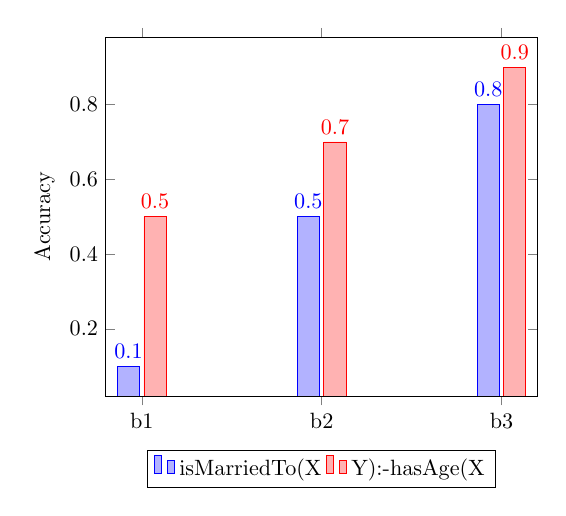
\begin{tikzpicture}[scale=0.8]
\begin{axis}[
    ybar,
    enlargelimits=0.10,
    legend style={at={(0.5,-0.15)},
      anchor=north,legend columns=-1},
    ylabel={Accuracy},
    symbolic x coords={b1,b2,b3},
    xtick=data,
    nodes near coords,
    nodes near coords align={vertical},
    ]
\addplot coordinates {(b1,0.1) (b2,0.5) (b3,0.8)};
\addplot coordinates {(b1,0.5) (b2,0.7) (b3,0.9)};
\legend{isMarriedTo(X,Y):-hasAge(X,Z) , isMarriedTo(X,Y):-hasAge(X,Z)hasChild(X,A)}
\end{axis}
\end{tikzpicture}
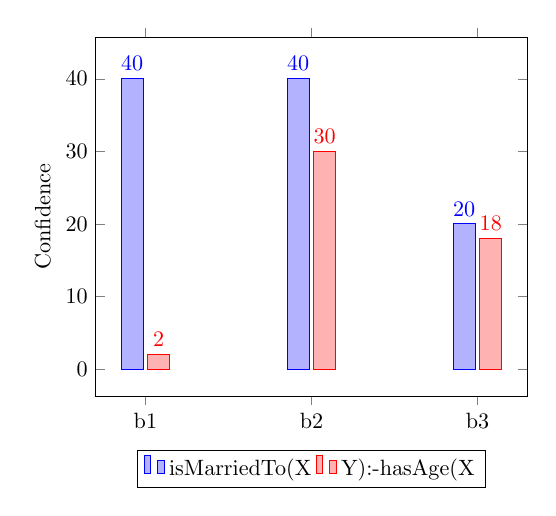
\begin{tikzpicture}[scale=0.8]
\begin{axis}[
    ybar,
    enlargelimits=0.15,
    legend style={at={(0.5,-0.15)},
      anchor=north,legend columns=-1},
    ylabel={Confidence},
    symbolic x coords={b1,b2,b3},
    xtick=data,
    nodes near coords,
    nodes near coords align={vertical},
    ]
\addplot coordinates {(b1,40) (b2,40) (b3,20)};
\addplot coordinates {(b1, 2) (b2,30) (b3,18)};
\legend{isMarriedTo(X,Y):-hasAge(X,Z), isMarriedTo(X,Y):-hasAge(X,Z)hasChild(X,A)}
\end{axis}
\end{tikzpicture}

Adding a given predicate to the rule might not bring any gain or even loss in accuracy to the base-rule, but when
bucketing per age, present a different accuracy and support distribution and might even produce gain in accuracy for
some specific buckets.

Nevertheless, adding a predicate with no correlation to the rule might not generate any gain. Thus, it's necessary to
carefully choose the relations and eventual constants and discard the ones with no correlation to the rule.  

\section{Contributions}
In this thesis, we propose a pre-processing step to build a graph we call \graphname for each numerical property we want
to for interesting intervals. In each graph, that has a numerical property as root, we first query the examples
distribution on the numerical attribute, and build a histogram by splitting them into \emph{k} buckets. Subsequently, we
pick a set of \emph{c} categorical properties that can be joined with the root, extract the frequencies histogram and
analyze how the distribution of sub-population created by joining them with the root is affected. Afterwards, we try to
combine the categories and check whether they still produce interesting sub-populations creating a lattice, like in
frequent set mining apriori algorithm.

We discuss the pruning opportunities and also evaluate different heuristics and interestingness measures and their
efficiency in finding rules with numerical intervals. 

\begin{comment}
In a clause containing a numerical attribute in the body, we can obtain a support and accuracy as well as support value
for each of the buckets. Therewith, we can search the most interesting intervals that satisfies the support and accuracy
thresholds
\end{comment}

With information about different examples distributions contained in the generated lattice, once we add one of the root
properties during the core ILP algorithm, we can then search for the most interesting categorical properties that could
result in different accuracy distributions. For every categorical property we can also suggest the most interesting
constants and other categorical properties to be combined in a subcategory of both.

\section{Outline}

\begin{comment}
 The remainder of this thesis is structured as follows. In
Chapter~\ref{ch:technical_background}, we provide technical background on
MapReduce and BigTable. In Chapter~\ref{ch:related_work}, we present a
summary of previous work in the areas of duplicate and near-duplicate detection,
information retrieval on web archives, and MapReduce applications in graph
processing. Following that, we state our problem and describe solutions in
Chapter~\ref{ch:redundancy_control}. In Chapter~\ref{ch:mapreduce_impl}, we
describe an implementation of our solution using the MapReduce framework. In
Chapter~\ref{ch:experiments}, we present our experimental results. We conclude
this thesis and outline directions of future research in Chapter~\ref{ch:future_work}.
\end{comment}
 % Introduction

\chapter{Related Work}
\label{rw:intro}

\section{Logic Programming}
\section{Inductive Logic Programming}
\section{Mining Opimized Rules for Numberic Attributes}

\cite{Brin99miningoptimized}

\section{Minimum Description Length}

\cite{DBLP:conf/sac/CaldersGPR09}

\section{Semamtic Web}
\section{Linked Open Data} % Related Work

\chapter{\graphname}
\label{ch:intro}

The idea is to build during preprocessing a graph inspired in the Itemset Lattice that describes the influence of different categorical relations on a given numerical attribute's distribution. We call such graph a \graphname.  To illustrate the idea, let's analyze a simple real-world example with the \emph{hasIncome} relation. If we have two categorical relations, one strongly correlated to income, e.g. \emph{hasEducation}, and one uncorrelated (or very weakly correlated), e.g. \emph{wasBornInMonth}.

Let's assume that for the relation \emph{wasBornInMonth(x,y)} we have the 12 months from the Gregorian Calendar as constants and for \emph{hasEducation(x,y)} we can have 10 different categorical constants for \emph{y}: ``Preschool, ``Kindergarten, ``ElementarySchool'', ``MiddleSchool'', ``Highschool'', ``Professional School'', ``Associate's degree'', ``Bachelor's degree'', ``Master's degree'' and ``Doctorate degree''. 

It's expected that the income distribution will be roughly the same for people born in any of the months, whereas for different education levels, e.g. Elementary School and Doctoral Degree, their income distribution are expected to be different between them and different from the overall income distribution.

In a further step, we try to join every possible pair of categorical relations and including the constants. For the given example with the relations \emph{hasEducation} and \emph{wasBornInMonth} we would then create the nodes:

  \emph{hasIncome(x,y)wasBornInMonth(x,``January''),hasEducation(x,``Preschool'')} \newline
  \emph{hasIncome(x,y)wasBornInMonth(x,``January''),hasEducation(x,``Kindergarten'')} \newline
  \dots \newline
  \emph{hasIncome(x,y)wasBornInMonth(x,``January''),hasEducation(x,``Doctorate Degree'')} \newline

  \emph{hasIncome(x,y)wasBornInMonth(x,``February''),hasEducation(x,``Preschool'')} \newline
  \emph{hasIncome(x,y)wasBornInMonth(x,``February''),hasEducation(x,``Kindergarten'')} \newline
  \dots \newline
  \emph{hasIncome(x,y)wasBornInMonth(x,``February''),hasEducation(x,``Doctorate Degree'')} \newline
 
  \dots \newline

  \emph{hasIncome(x,y)wasBornInMonth(x,``December''),hasEducation(x,``Preschool'')} \newline
  \emph{hasIncome(x,y)wasBornInMonth(x,``December''),hasEducation(x,``Kindergarten'')} \newline
  \dots \newline
  \emph{hasIncome(x,y)wasBornInMonth(x,``December''),hasEducation(x,``Doctorate Degree'')} \newline


Based on this idea, we basically check how different categorical relations affect a numerical distribution. Such information, together with other measures like support, provides valuable cues on what categorical attributes and what categorical constants might be the most interesting to be added to the hypothesis in the core ILP algorithm.

\section{Categorical Relation Definition}

In this section, we formally define a categorical relation as used in the \graphname. 

First of all, a candidate relation must be joined with root relation's \ord{1} argument (assuming that the numerical attribute is in the \ord{2} argument). 

A candidate categorical relation $r(x,y)$, should be equivalent a non-injective function:

$r(x,y) \equiv f : X \rightarrow Y ,\, s.t. |Y|<|X| $ and $  |Y|=n ,\, n>1 \newline $
$\nexists \, g : Y \rightarrow X ,\, s.t. f(g(x))=x ,\, \forall x \in X$

We can define subsets of $X_i \in X$, with which of them belonging to one category $y_i \in Y$:

$X_i \subset X ,\, s.t. X_i = \{x \in X \,|\, f(x)=y_i ,\, y_i \in Y\} \newline $
$X = \bigcup_{i=1}^{n} X_i $ and $ X_i \cap X_j = \emptyset ,\, \forall i,j \in [1,n] ,\, i \neq j$

We can also broaden this definition by composing functional relations to a categorical or multiple categorical relations:

If we have:

$r_1(x,y) \equiv f_1 : X \rightarrow Y$ (categorical or not) \newline
$r_2(y,z) \equiv f_2 : Y \rightarrow Z$ (categorical relation)

Then,

$r'(x,z) \equiv f : X \rightarrow Z$, where $r'(x,z)=r_2(f_1(x),z)$ is also categorical


Numerical relations can also be turned into a categorical, by simply applying a bucketing function that maps a numerical domain into a finite set of $k$ buckets:

$b: \mathbb{N} \rightarrow B$, where $B=\{b_1,b_2,\dots ,b_k \}$

So a numerical relation:

$r(x,y) \equiv f : X \rightarrow \mathbb{N}$ 

combined with a bucketing function $b$, $r'(x,b(y))$ would be categorical

(Then talk about non-categorical relations as categorical by considering its presence/absence)

\section{Support}

As described in (\cite{LavracDz94}), in top-down ILP every refinement causes the support to decrease, therefore we know that for every node in the \graphname, its support will be greater or equal than any of its children, so support is a monotonically decreasing measure so we can safely prune a node that doesn't reach the minimum support threshold.


\subsection{Independece between Nodes}

By simplicity, we assume that every possible pair of categorical relations are independent and we search for evidence to prove the contrary.

For 2 nodes to be joined, they must have a common parent, i.e. two nodes at level $l$ (with $l+1$ literals) are joinable if they share $l$ literals. Therefore, it's straightforward to calculate the conditional probabilities of each of the joining nodes given the common parent, and estimate the frequency distribution for the conditional independence case.

If we are joining hasEducation()...

For every bucket $b_i$ in the frequency histogram, we can calculate the conditional probability $p_i(n_1|p)$ and $p_i(n_2|p)$ assuming conditional independence given $p$ in order to estimate $\hat{h_i}(n1,n2)$:

\begin{equation}
\begin{split}
 p_i(n_1|n_2,p) &= p_i(n_1|p) \\ 
 &= \cfrac{h_i(n_1)}{h_i(p)} \\ 
 p_i(n_2|n_1,p) &= p_i(n_2|p) \\ 
 &= \cfrac{h_i(n_2)}{h_i(p)} \\ \\ 
 \hat{h_i}(n_1,n_2) &= p_i(n_1|n_2,p)*p_i(n_2|p)*h_i(p) \\ 
 &= p_i(n_1|p)*h_i(n_2) \\ 
 \hat{h_i}(n_1,n_2) &= p_i(n_2|n_1,p)*p_i(n_1|p)*h_i(p) \\ 
 &= p_i(n_2|p)*h_i(n_1) 
\end{split}
\end{equation}

After that, we query the actual frequency distribution on the Knowledge Base and do an Pearson's chi-squared independence test. As null hypothesis and alternative hypothesis we have:

\begin{center}
  $H_0$ = \emph{$n_1$ and $n_2$ are conditionally independent given their common parent $p$} 
  $H_1$ = \emph{$n_1$ and $n_2$ are conditionally dependent given their common parent $p$} 
\end{center}

Number of degrees of freedom is the number of buckets minus one:

\begin{center}
 $df=k-1$
\end{center}

We calculate the $\chi^2$ value:

\begin{equation}
 \chi^2=\sum_{i=1}^{k} \cfrac{(h_i - \hat{h_i})^2}{\hat{h_i}}
\end{equation}

\cite{Jaroszewicz02pruningredundant}

\section{Heuristics}

Then it's possible to obtain the p-value and check whether there's enough confidence to reject the null hypothesis $H_0$.



\chapter{Algorithmic Framework}
\label{af:intro}

\section{Knowledge Base Backend}

For storing and retrieving RDF data we use RDF3X \cite{Neumann:2010:RES:1731351.1731354}. It has the advantage of being specialized and optimized for RDF data, using a strong indexing approach with compressed B$^+$-Tree indices for each of six permutations of \emph{subject (S)}, \emph{predicate (P)} and \emph{object (O)}: \emph{SPO},\emph{SOP},\emph{OSP},\emph{OPS},\emph{PSO} and \emph{POS}.

RDF3X particularities...

\section{Preprocessing}

\subsection{\graphname}

\subsubsection{Graph Node}

Every node essentially contains the following attributes:

\begin{itemize}
 \item Set of pointers to parent nodes
 \item Set of pointers to child nodes
 \item Set of pointers to constant nodes
 \item Histogram with facts distribution over root numerical property
\end{itemize}


\subsubsection{Building the Correlation Lattice}

For building the \graphname, we start with the root node, which has a numerical property as literal and no constants assigned, e.g. \emph{hasIncome(x,y)}. We then query the  distribution of positive examples over the property in the whole Knowledge Base.

\begin{center}
 \emph{SELECT COUNT ?y WHERE \{ ?x <hasIncome> ?y \} GROUP BY (?y)}
\end{center}

It's also necessary to specify the bucketing technique and the number of buckets in order to extract the histogram from the obtained query results. These buckets are used to build the histograms of all nodes in the graph.

Afterwards, we select the the categorical properties that will be used in the lattice. For each of the selected properties, we join them with the root numerical property (for simplicity we'll assume all the categorical properties are joined with both \ord{1} arguments) and we query the distribution again. In the first level, it's necessary to extract a histogram for each of the categorical constants in the selected properties. Therefore, it's a good strategy to group the results also by these categorical constants so If we select \emph{hasEducation} for example, we would then fire the following SPARQL query:

\begin{center}
 \emph{SELECT COUNT ?z ?y WHERE \{ ?x <hasIncome> ?y . ?x <hasEducation> ?z \} GROUP BY (?z,?y)}
\end{center}

With such query, it's possible to extract a histogram for the node \emph{hasIncome(x,y)hasEducation(x,z)} and its correspondent constants. 

\subsubsection{Searching Rules in Correlation Lattice}

In the \graphname itself, it's possible to extract valuable rules. Given its characteristic of all the relations being joined on the same root argument, those rules represent how different categories are related along root's numberical constants.

For every non-root node in the \graphname, any of its parents can be seen as rule's body and the remaining literal as head, e.g.:

Let's denote $a_i$ as a relation $a(x,y)$ with constants $A_i$ for $y$, so for example $a_1 \equiv a(x,A_1)$:

For the node $r a_1 b_1 c_1$ with parents $r a_1 b_1$, $r a_1 c_1$ and $r b_1 c_1$, we can extract and easily evaluate three rules:

\begin{math}
Rule_1 : \quad a_1 \leftarrow b_1 c_1 r \\ 
\quad supp_i(Rule_1) = h_i(r a_1 b_1 c_1) \\
\quad \quad acc_i(Rule_1) = \frac{h_i(r a_1 b_1 c_1)}{h_i(r b_1 c_1)} \\ \\
Rule_2 : \quad b_1 \leftarrow a_1 c_1 r \\
\; supp_i(Rule_2) = h_i(r a_1 b_1 c_1) \\
\; acc_i(Rule_2) = \frac{h_i(r a_1 b_1 c_1)}{h_i(r a_1 c_1)} \\ \\
Rule_3 : \quad c_1 \leftarrow a_1 b_1 r \\
\; supp_i(Rule_3) = h_i(r a_1 b_1 c_1) \\
\; acc_i(Rule_3) = \frac{h_i(r a_1 b_1 c_1)}{h_i(r a_1 b_1)} \\
\end{math}

Subsequently we can analyze the frequency and confidence distributions and determine whether any of the rules are
interesting, using any of the techniques discussed in [???] and find possible interesting intervals.

\subsubsection{}

% Substitution for constants only in categorical relations, query by support
% When categorical joined to numerical property (without range) existent in \graphname query graph for constants
% 



 % Data Model

%\input{./Chapters/Chapter5} % Information Extraction

%\input{./Chapters/Chapter6} % Context-Aware Ranking

%\input{./Chapters/Chapter7} % Implementation

%\input{./Chapters/Chapter8} % Experiment

%\input{./Chapters/Chapter9} % Conclusion

%% ----------------------------------------------------------------
% Now begin the Appendices, including them as separate files

\addtocontents{toc}{\vspace{2em}} % Add a gap in the Contents, for aesthetics

%% ----------------------------------------------------------------
%\lhead{\emph{List of Figures}}  % Set the left side page header to "List if Figures"
\listoffigures  % Write out the List of Figures

%% ----------------------------------------------------------------
%\lhead{\emph{List of Tables}}  % Set the left side page header to "List of Tables"
\listoftables  % Write out the List of Tables

\appendix % Cue to tell LaTeX that the following 'chapters' are Appendices

%\input{./Appendices/AppendixA}	% Appendix Title

%\input{./Appendices/AppendixB} % Appendix Title

%\input{./Appendices/AppendixC} % Appendix Title

\addtocontents{toc}{\vspace{2em}}  % Add a gap in the Contents, for aesthetics
\backmatter

%% ----------------------------------------------------------------
\label{Bibliography}
\lhead{\emph{Bibliography}}  % Change the left side page header to "Bibliography"
\bibliographystyle{unsrtnat}  % Use the "unsrtnat" BibTeX style for formatting the Bibliography
\bibliography{Bibliography}  % The references (bibliography) information are stored in the file named "Bibliography.bib"

\end{document}  % The End
%% ----------------------------------------------------------------